\chapter[Passwords -- A User Perspective]{Passwords -- \\
	A User Perspective}\label{chap:rw:user_perspective}
%lingo: arduous

``but his thoughts were so full of the great riches he should possess, that he could not think of the word to make it open, but instead of `Sesame,' said, `Open, Barley!' and was much amazed to find that the door remained fast shut. He named several sorts of grain, but still the door would not open, and the more he endeavoured to remember the word `Simsim,' the more his memory was confounded, and he had as much forgotten it as if he had never heard it mentioned.'' (Kasim's predicament in \textit{Ali Baba and the Forty Thieves}) \todo{this could be the opening of the chapter / fancychapter}

%alternatively: this: [King Roland has given in to Dark Helmet's threats, and is telling him the combination to the "air shield"] Roland : One. Dark Helmet : One. Colonel Sandurz : One. 
% Roland : Two. Dark Helmet : Two. Colonel Sandurz : Two.
%Roland : Three.
%Dark Helmet : Three.
%Colonel Sandurz : Three.
%Roland : Four.
%Dark Helmet : Four.
%Colonel Sandurz : Four.
%Roland : Five.
%Dark Helmet : Five.
%Colonel Sandurz : Five.
%Dark Helmet : So the combination is... one, two, three, four, five? That's the stupidest combination I've ever heard in my life! That's the kind of thing an idiot would have on his luggage!

Morris and Thompson were already concerned with user behavior regarding passwords in 1979 \cite{Morris1979PasswordSecurity}. They identified that users choose predictable passwords and that this can be leveraged for attacks. So, they suggested enforcing a certain minimum password length (six characters). At the time, the users were mostly professionals that received training to operate computers and could thus also have been trained to pick less predictable passwords \cite{Maguire2012YouOnlyLiveTwice}. But as computers were introduced to a larger audience, more people were exposed to password authentication. Naturally, this also induced a growing number of attacks, and it is increasingly difficult for users to defend themselves against them (see. Section \ref{sec:rw:attack_vectors}). Nowadays, password policies are in place that require not only a minimum of eight characters, but also mandate mixed-case letters, digits and special symbols to start with. The HCI community noticed the users' struggle in the 1990s and that we can -- and should -- design authentication systems with usability in mind. Perhaps, one of the breaking points where a new school of thought turned up in the literature was a paper by Adams and Sasse in 1999 \cite{Adams1999UsersEnemy}. The central and novel theme in there was a shift from \textit{fixing} the user to \textit{acknowledging} user behavior and designing for it. The paper managed to see over 1500 citations as of writing this.

This chapter looks at the literature that mostly came after this seminal work. It discusses the users' problems, solutions, feelings, and opinions about using passwords. An essential goal is to give the reader an empathetic perspective and provide background information to understand why it seems hard to come up with viable solutions to make users' lives less frustrating. To get there, we first take a brief look at conducting user research with passwords. Hereafter we disseminate typical coping strategies and solutions. The chapter concludes with a comment on the discourse that has been going on between the very different schools of thought about passwords. 

%Each person who gets in contact with the Internet will at some point create a password.

% Everyone develops their own strategy how to do this and how to cope with passwords, probably already in early teenage years \cite{VonZezschwitz2013SurvivalShortest}. These strategies however are not unique and show macroscopic commonalities, which became evident after the first large-scale password leaks. 

%Important: Under coping strategy, we also understand the selection process, because choosing a weak password over a strong one is also one way to \textit{cope} with the large number of passwords and the memorability burden. (make sure to mention this in the general introduction already.)

\section{Methodology: Running Password Studies}\label{sec:rw:methodology}
% not relevant: how to measure password strength. solely focus on the ``HOW'' of data collection
Before we report on insights about user behavior regarding passwords, we take a look into running studies that focus on passwords. There are two central aspects that make collecting data particularly challenging: acting ethically and maintaining high ecological validity of the data. In fact, these two goals create an area of tension that demands a critical selection of methods. Komanduri \etal note that ``ideally, password studies would be conducted by collecting data on real passwords created by real users of a deployed system'' \cite{Komanduri2011OfPasswordsAndPeople}. But this would mean that researchers obtain access to the user accounts that were under investigation. This is ethically questionable \cite{Egelman2012ItsNotStealing}. Maybe the researchers themselves are benevolent, but the data is precious and thus could bring attackers to the scene. Since absolute security can barely be guaranteed, it is best to avoid that users disclose their actual credentials during a user study to the researchers.

\subsection{General Considerations for User Studies as Data Source}
If we cannot collect the users' real password in its original form, what is the best way to measure, e.g., cause and effect of novel interventions? There are several alternatives. 
% first solution: have people create a new one. 
\subsubsection{Password Creation Tasks} First, one asks participants to create a new password during the user study and stores these passwords as part of the dataset. This approach resolves the issue of real-world password disclosure, but introduces a number of problems.
% ethical dilemma #1: do people know that their passwords are studied? 
Studies should be ethical and thus transparent for the most part. Hence, the study topic should be known to the participants. However, if participants know that their passwords are studied, this could induce protective reactions to prevent giving hints about their real passwords at all. In that case, the participants' selection strategy does not resemble much to their real-world behavior and thus the ecological validity of the data is low \cite{Shay2012CorrectHorseBatteryStaple}. 
% give a realistic risk
Although it appears trivial, Fahl \etal suggest that in this scenario, asking the participants whether they had acted like they normally would is a suitable indicator that helps in weighting the data \cite{Fahl2013EcologicalValidityPasswordStudy}. It is also recommendable to give users a specific scenario that allows them to immerse themselves in the task. Komanduri \etal argue that having participants create passwords for fictional email accounts leads to more authentic behavior \cite{Komanduri2011OfPasswordsAndPeople}.
% ethical dilemma #2: sharing the collected data. 
Some users, however, are less protective and provide one of their real passwords regardless of the instruction (e.g. 26.5\% in Fahl \etal's study \cite{Fahl2013EcologicalValidityPasswordStudy}). The result is the same as if the purpose of the study was concealed through an act of deception, which is occasionally done in psychology studies (for a discussion see \cite{Tai2012Deception}). For example, it can suffice to tell participants a convincing \textit{cover story}, e.g. that the purpose of the study is to do a usability test of a social networking site, which also happens to involve an account setup process. The data would be ecologically valid because it removes observer-expectancy and other biases. For the researchers, however, it is extremely difficult to tell ``real'' passwords and ``new'' passwords apart. Thus, phishing or man in the middle attacks are sometimes carried out. Haque \etal conducted a laboratory study where they told participants a cover story to create new accounts for popular websites \cite{Haque2014Hierarchy}. The websites, however, were re-created by the researchers and stored the passwords on their own servers instead of performing actual registrations. Egelman \etal used a proxy server to intercept traffic between the users and a real online portal \cite{Egelman2013DoesMyPasswordGoUpToEleven}. They also altered the websites to communicate their cover story that the password had expired. This, however, creates an ethical conundrum, if the dataset is published along with the paper. To allow others to verify that research is valid, reliable, and generalizable, a published dataset is desirable, but in Egelman \etal or Haque \etal's study this would put real user accounts at risk.
% ethical dilemma #3: sharing cracking algorithms.
Much in the same vein, sharing research about successfully attacking passwords produces a similar dilemma. For instance, one can put forward new cracking approaches (e.g. \cite{Marechal2008AdvancesPWCracking, Narayanan2005FastDictionaryAttacks, Schmidt2013Pitfalls, Weir2009PCFG}) that potentially affect common strength metrics (see Section \ref{sec:rw:pw_strength_metrics}) -- but attackers also benefit from this kind of knowledge. From an HCI perspective, one can also unfold how users select passwords, which allows optimizing cracking efficiency \cite{Weir2010MetricsPolicies, Wheeler2016zxcvbn}. 


% SOLUTIONS TO ETHICAL PROBLEMS
There are several methods to avoid acting unethically in studies where users are required to create passwords. 
% IRBs
First of all, studies involving human subjects are assessed by an \gls{IRB}, especially in the United States. This is done to ensure an ethical study design that is unlikely to cause participants any harm. The \gls{IRB} might mandate a thorough debriefing of participants and meticulous documentation of the experiment. In Europe, however, password studies are less commonly evaluated by an IRB (or authors fail to mention the process in their papers) \ar. 
% Do not publish data sets.
Secondly, one can refrain from releasing the data set, even if user names are removed. In fact, almost all publications on passwords collected during a user study omit publishing the corresponding data set. Only the abstract analysis is published and this is a widely-accepted standard practice, despite the questionable reliability. 
% Differential privacy.
A rather novel approach that reduces the likelihood of made-up data relies on the idea of publishing differentially private data sets. Here, algorithmically generated noise, which is indistinguishable from the orignal data, is added to the data set to preserve privacy of users. For password frequency lists, passwords could be mangled and extended by generated passwords that resemble real ones. Adversaries lack information whether the data is usable as signal or noise.
This way, Blocki \etal managed to release a private frequency list of passwords at Yahoo that Bonneau had already anonymously analyzed in \cite{Bonneau2012ScienceOfGuessing}. 
% Encryption
Moreover, instead of collecting newly generated passwords in plain text, it is possible to store a hashed version. For instance, Wash \etal had participants install a browser extension that logged all form submits that included a password field \cite{Wash2016UnderstandingPasswordChoices}. To study reused passwords, they hashed and sent them over a secure connection to their servers. As long as a slow hash function and a strong salt are used, this approach is uncritical. However, it merely allows observing if the hashes match on several sites.
% Meta data
Finally, as a last option to collect password data, researchers can log meta-data instead of passwords. For instance, Von Zezschwitz \etal used a ``meta password'' that described the participants' actual passwords \cite{VonZezschwitz2013SurvivalShortest}, but which was insufficient to reconstruct the original. This can include the number of characters, upper-/lowercase letters, digits, and even proactive strength estimations. To collect the data, participants in von Zezschwitz \etal's study were provided with an offline password analysis tool. They entered their password into that and copy-pasted the result of the analysis into the questionnaire form. If one does not want to examine the passwords qualities, this approach is absolutely feasible. Florêncio and Herley used a similar approach for the large-scale data collection with around 500000 participants to avoid running into privacy issues \cite{Florencio2007LargeScaleStudyPasswordHabits}. The information transmitted to the logging server was pseudonymized and contained only meta features. The only downside is that one cannot run further analyses on the passwords, e.g. if a new strength metric is considered.

% second solution: SELF REPORT instead of the task to create a password
\subsubsection{Retrospective Self Report}
If one wants to refrain from having users create a new password, one can study their past behavior in different ways. In its simplest form, participants are simply asked to describe how they create passwords. Stobert \& Biddle did this in extensively to create the Password Life Cycle model \cite{Stobert2014PasswordLifeCycle} (see Section \ref{sec:rw:user-behavior}). Ur \etal used interviews to find out what users do to make their passwords stronger \cite{Ur2015PWCreationLab}. Das \etal found out through retrospective interviews that social contacts have a strong impact on users' security decisions \cite{Das2014EffectSocialInfluenceSecuritySensitivity}. Most commonly, however, typical online surveys feature a number of questions about personal behavior and attitudes, e.g. \cite{Adams1997MakingPWsSecureAndUsable, Gaw2006PasswordManagement, Kuo2006HumanSelectionMnemonic,Riley2006WhatUsersKnowWhatTheyDo, Shay2010EncounteringPasswordRequirements}. Questions about passwords are easy to implement in a survey and respondents can always choose how much they want to share. However, one has to stay aware that social desirability lowers the reliability of the data: since the media also to their part in shaming users for picking ``bad'' passwords, people may respond dishonestly about their password behavior. Many people are uncomfortable admitting their password is as simple as 12345. Another problem results from fading memories. Since most users have more than one password, it might be difficult for them to recall the correct past behavior. However, not only password studies suffer from this bias, but any study involving self report in general. 

\subsubsection{Principles}
From user research in \acrshort{USEC} of the past decades, Krol \etal derive a set of general principles that researchers ought to consider when conducting experiments in security and privacy \cite{Krol2016ExperimentDesign}. We can integrate password studies in there:
%\vspace*{-0.5cm}
\paragraph{Primary Task} Creating a password should not be the sole task in the study. Instead, participants should achieve a primary task by authenticating with passwords, e.g. using a new system for a period of time \cite{Brostoff2000PassfacesEvaluation}. The reasoning behind this principle is that security tasks are secondary tasks and this constraint needs to be reflected in the experiment. However, re-focusing on a separate primary task is not always possible, e.g. in surveys. 
\vspace*{-0.5cm}
\paragraph{Realistic Risk} Users should be able to realistically estimate the risk for secure interactions. As mentioned above, Komanduri \etal suggest carefully selecting real-world scenarios to achieve this \cite{Komanduri2011OfPasswordsAndPeople}.
\vspace*{-0.5cm}
\paragraph{No Priming} Whenever human behavior is studied, experiments should avoid influencing and biasing participants with certain information. This avoids unnatural behavior.  
\vspace*{-0.5cm}
\paragraph{Double Blind Experiments} If possible, the person carrying out the actual experiment should be involved in the planning and design of the study. Moreover, the participants should not know the details of the study, either. On the experimenter side, unconscious bias and influence is mitigated, and participants also do not know the ``treatment'' they receive (if any). Although this is a desirable goal, there is little evidence that experiments are usually carried out in this way. 
\vspace*{-0.5cm}
\paragraph{Context Definition} To increase internal validity, it is necessary to define the terms \textit{threat model}, \textit{security}, \textit{privacy}, \textit{usability}, depending on which are relevant for the study. A precise definition avoids misunderstanding and improves transparency, credibility, and trustworthiness of the experiment.\\ 

\noindent These principles can serve as a rough quality assessment of presented research, although in many instances, not all principles will be fully addressed.

% briefly show the benefits and drawbacks of each method. 
%TODO maybe some Usable Security book already has this? look into garfinkel/cranor book...
\subsection{Analyzing Password Leaks and (Semi-)Public Data}
% frequency lists are a source of data
Instead of users creating new passwords, it is possible to make inferences about their behavior from already existing data (for an overview see Table \ref{tab:rw:password_leaks}). Password frequency lists are readily available on the Internet \footnote{An example repository containing a wide range of leaked passwords is available under \url{https://github.com/danielmiessler/SecLists/tree/master/Passwords} \la{09.01.2018}}. The sources can often be traced back to illegal attacks, which makes the use of such data somewhat questionable. However, it is a widely accepted method to contrast real-world and study behavior. The data set that has probably been studied the most originates from a breach at RockYou, a software development firm specialized at games for social networks. In 2009, an attacker used an SQL injection to download around 32 Million plain-text passwords. For instance, Veras \etal visualized semantic properties of passwords in this dataset and highlight the high occurrence of dates in there \cite{Veras2012VisualizingSemanticsPasswords}. Wheeler relied on it to build the zxcvbn password strength estimation system. More often, though, these data sets serve as training data for password guessability benchmarks. Weir \etal took the RockYou passwords to train their \gls{PCFG} which served as a demonstration that entropy is not a feasible strength metric for user-chosen passwords. Afterwards, it was integrated into the training set of \gls{PGS}. \gls{PGS} is mostly used to gauge passwords collected through a user study, e.g. under different policies \cite{Shay2016DesigningPasswordPolicies} or interventions \cite{Ur2017DataDrivenPWMeter}. In conclusion, publicly leaked data sets can often serve as ground truth for studies that aim to provide new insights.  

%
% PASSWORD LEAKS, label: tab:rw:password_leaks
% password leaks

% Table generated by Excel2LaTeX from sheet 'leaked datasets'
\begin{table}[htbp]
  \centering
  \caption{\label{tab:rw:password_leaks} Example password leaks of the past five years. Some of the data served security researchers to analyze user behavior and create more effective strength estimation algorithms.}
    \begin{tabular}{lrrl}
    \textbf{Data Source} & \textbf{\# PWs} & \multicolumn{1}{l}{\textbf{Year}} & \multicolumn{1}{l}{\textbf{Literature}} \\
    \midrule
    \midrule
    RockYou & 32 M  & 2009  & \todo{add references that used the data.} \\
    LinkedIn & 164 M & 2016  & \todo{provide references for the info in this table} \\
    Dropbox & 68 M  & 2012  &  \\
    MySpace & 360 M & 2013  &  \\
    ebay  & 145 M & 2014  &  \\
    Adobe & 36 M  & 2013  &  \\
    Yahoo & 1 B   & 2013  &  \\
    \end{tabular}%
\end{table}%

% https://pgs.ece.cmu.edu/ at the bottom has a couple of statistics what kind of data they use.
% DeCarnedeCarnavalet2015PasswordMeters too

%
%

\subsection{User Study Methods in Password Research}
Research in \acrshort{USEC} takes advantage of the toolbelt of \acrshort{HCI} research in general. In the following, the most common methods for password studies are portrayed.
\paragraph{Laboratory studies}
% not focused on password: \cite{Sotirakopoulos2011ReplicationSSLWarnings}
To gain the greatest control over experimental parameters, laboratory studies are the go-to method. Both qualitative and quantitative studies are carried out in the lab, with a slight surplus of qualitative studies. Among the most common methods, one finds (semi-)structured interviews (\cite{Adams1997MakingPWsSecureAndUsable,Gaw2006PasswordManagement, Stobert2014PasswordLifeCycle, Ur2015PWCreationLab, Weirich2001PrettyGoodPersuasion}) and usability testing (\cite{Egelman2013DoesMyPasswordGoUpToEleven,Forget2007HelpingUsers,Forget2015CYOA,Gross2016CognitiveDepletion,Imran2015PWsAdultsChildren, McCarney2012Tapas,Mcevoy2016ContextualizingMnemonicPhrase,Ruoti2015AuthenticationMelee, Yang2014EntryAffectsPasswordSecurity,VonZezschwitz2014HoneyIShrunkTheKeys}). Password memorability can be studied in the lab (\cite{Egelman2013DoesMyPasswordGoUpToEleven,Fahl2013EcologicalValidityPasswordStudy,Forget2008MemorabilityPersuasivePasswords,Mcevoy2016ContextualizingMnemonicPhrase,Yan2004PasswordMemorabilitySecurity}). Studying short-term recall usually follows a mental-rotation task (e.g. \cite{Kraus2017Emoji,Yang2014EntryAffectsPasswordSecurity}). Long-term memorability studies in the lab are less common, because they require participants to return to the lab, which may be too bothersome for many. For alternative authentication schemes, this may, however, be the only option. 

Although technically it is not a ``lab'' environment, café studies sometimes are closely related to lab studies. Von Zezschwitz \etal collected qualitative and quantitative data on participants' past password behavior by inviting customers in a café to join them for a free coffee \cite{VonZezschwitz2013SurvivalShortest}. The experimenter has almost as much control as in a lab to answer certain research questions. Only the surroundings may distract somewhat. Other methods like participatory design / co-creation (\cite{Coventry2014SCENEBehavioralNudges,Read2009UnderMyPillow}) and focus groups (\cite{Eargle2015YouCanDoBetter,Hang2015Dissertation,Harbach2016HardLockLife,Singh2007PasswordSharing}) are possible, but less frequently reported than interviews and usability tests. A common drawback of lab studies lies in the high costs, time consumption to carry them out, smaller sample sizes, and reduced ecological validity.

\paragraph{Field-Studies}
Field studies for password research come in many flavors. 
% regular online surveys (no mTurk)
\textbf{Online surveys} are among the most common methods used in the field (\cite{Gaw2005ReuseRecycle,Halevi2013PilotStudyPersonality,Haque2014Hierarchy,Huh2017TooBusy, Kuo2006HumanSelectionMnemonic,Mazurek2013Measuring,Riley2006WhatUsersKnowWhatTheyDo, Violettas2014PasswordsAvoidGreece}), due to their lower cost and comparatively easy implementation. Other advantages like increased sample size and more diversity in the data speak in favor of online surveys. Survey tools like surveymonkey.com come in handy, but usually lack seamless integration of interactive prototypes. If a prototype should be evaluated through a survey, however, one has to either implement the entire survey structure or redirect participants from the survey platform to the prototype and back. Surveys are also the weapon of choice if there is an opportune moment that is worth studying. Mazurek \etal took the opportunity to distribute online questionnaires after a new password policy was introduced at \acrshort{CMU} \cite{Mazurek2013Measuring}. Fahl \etal profited from a similar situation at Leibniz-University Hannover, and Renaud \etal could even distribute surveys on the same topic across multiple years in this way \cite{Renaud2017LessonsLearnedNudges}. Interestingly, there does not seem to be a special, standardized survey construct to measure the usability, respectively user experience, of password systems. Other \gls{HCI} sub-fields more frequently use, for example, the NASA-TLX, \gls{PANAS} or AttrakDiff constructs to establish comparability with other studies. Notable exceptions were reported by Kraus \etal, who used AttrakDiff to evaluate emoji-based authentication \cite{Kraus2017Emoji}. The NASA-TLX was used by Fraune \etal, \cite{Fraune2013UserCreatedPictures}, Sherman \etal \cite{Sherman2014UserGeneratedGesturesAuth}, and Yang \etal \cite{Yang2014EntryAffectsPasswordSecurity}. Lately, the \gls{SeBIS} gains more attention, because it serves as a self-assessment that can help the interpretation of actions taken during a user study  \cite{Egelman2015SeBIS, Egelman2016BehaviorEverFollows, Wash2016UnderstandingPasswordChoices,Wash2017SelfReport}.

% mTurk studies
A special kind of online studies that has been extensively used and propagated by \acrshort{CMU} researchers leverage \textbf{crowd-sourcing} platforms like the Amazon Mechanical Turk (\gls{mTurk})\footurl{https://www.mturk.com/}{10.01.2018}. Survey respondents are recruited by paying each one a small amount of money for a valid response. This way, increasing the sample size is straight-forward, if many users have already signed up on the platform and are eligible for the \acrfull{HIT}. Workers (known as ``turkers'') form an increasingly diverse population \cite{Ross2010WhoAreTurkers}, which is another benefit.
% mturk examples.
In password research, for instance, Kelley \etal's high-impact work on password guessability collected around 12000 passwords using \gls{mTurk} \cite{Kelley20012GuessAgain}. Ur \etal had participants rate the strength and memorability of a given set of passwords, which allowed them to identify certain misconceptions \cite{Ur2016PerceptionsPassword}. Mazurek \etal compared features of passwords created by turkers to real passwords of students and staff at their university \cite{Mazurek2013Measuring}. They take the large similarities of the two data sets as evidence that passwords created during an mTurk study are a reliable and valid data source, so there is no urgent need to analyze passwords of a deployed system. Shay wrote a PhD thesis specifically about evaluating password policies with crowd-sourced data \cite{Shay2015UsablePoliciesMTurk}. 
% slightly starting to address issues
In many cases, e.g. \cite{Shay2014CanLongPasswordsBeSecureAndUsable,Shay2016DesigningPasswordPolicies,Ur2017DataDrivenPWMeter}, the primary task is to create a fictional account or merely a password under certain constraints, which apparently violates Krol \etal's study principles \cite{Krol2016ExperimentDesign}. It is especially interesting that most studies are announced as some kind of password study, probably mandated by \glspl{IRB} . But Mazurek \etal's work demonstrates that this limitation is bearable. Moreover, studying the long-term memorability of passwords is facilitated, because participants can be invited to return through an internal, anonymous messaging system. It is also possible to create more complex study designs with mTurk, e.g. if multiple device types should be used by the turkers to create passwords \cite{Melicher2016UsabilityMobileTextPasswords}. 
% issues with mTurk studies
Despite the wide range of advantages, there are shortcomings of crowd-sourced approaches as with any study method. First, turkers are incentivized to complete as many HITs as possible on the platform to earn money. Thus, completing a survey by providing quick answers without reading the questions could lead to unreliable data. Instructional Manipulation Checks (IMCs) and attention check questions (ACQs) can mitigate this problem \cite{Oppenheimer2009InstructionalManipulationChecks, Peer2017BeyondTheTurk}. Turkers are only paid if the commissioner accepts the HIT as valid, thus IMCs and attention checks are useful indicators here. Moreover, as of now, the mTurk platform can only be used in certain countries, e.g. the USA or UK. European alternatives exist, but are not yet par in terms of user base, response times, and feature set \cite{Peer2017BeyondTheTurk}. 

% diary studies
Aside from surveys, \textbf{diary studies} about passwords have proven feasible in the past. Inglesant and Sasse found out through a diary study that employees struggle with frequent password changes, which might not have become evident using other study means \cite{Inglesant2010TrueCostOfUnusablePolicies}. Hayashi and Hong used this method to analyze password re-use across different computers, services, and organizations \cite{Hayashi2011DiaryStudyPWs}. Since password authentication is a secondary task, keeping a diary of authentication events helps participants provide reliable behavioral data. However, it requires much effort to continuously stay aware of one's actions to log them. To avoid that participants forget logging and other self-reporting bias \cite{Wash2017SelfReport}, it can be worthwhile to ask them small questions in situ. This method, known as \textbf{\gls{ESM}}, requests short responses either in predefined intervals or when the system detects a relevant event. ESM has not seen much attention in password studies on the web, but it authentication on mobiles was studied with this method \cite{Harbach2016HardLockLife}. Users carry their personal mobile with them almost all the time, so there is a high chance of successfully receiving the experience sample. ESM was also found useful for studies about security warnings in browsers \cite{Akhawe2013AliceInWarningland,Felt2016RethinkingConnectionSecurityIndicators}.

% automated logging
Perhaps, ESM is underused for password studies, because it is possible to automatically detect such events and survey the participants before and/or after the \textbf{automatic data collection}. Florêncio and Herley conducted one of the largest studies to date on password habits with this method \cite{Florencio2007LargeScaleStudyPasswordHabits}. Their intention was to find out among other things A) how often people type passwords, B) how many sites share a password C) how many distinct passwords a user has, and D) how the strong the passwords are. Working at Microsoft, they were granted to utilize the Windows Live Toolbar for Internet Explorer to collect in-the-wild data from up to 500,000 users during three months of running the collection. They conceived the method of protected password lists (PPL) to avoid intruding into people's privacy -- a kind of meta description of passwords which is sent to the logging server instead of the original password. It was thus not possible to trace the incoming data back to a specific user. However, there are a number of limitations this method. The authors point out that the anonymity of the incoming data-stream might have resulted in over-counting of entries. Also, it was not measured how long the actual password entries takes. If users only used regular dictionary words without any modification as their passwords, the key logging module of the toolbar would have recorded a password reuse event (PRE) every time the user entered that word -- also in regular online communication. Nevertheless, the fact that users are typically focused on their primary tasks, background logging helps to collect unbiased data with high ecological validity. 

% deployed systems
A final option to study passwords in the field is to collect and analyze them in an already deployed system (\textbf{in-situ evaluation}), which would be the ideal data source, according to Komanduri \etal \cite{Komanduri2011OfPasswordsAndPeople}. Brostoff and Sasse utilized a coursework system to evaluate Passfaces as alternative to passwords \cite{Brostoff2000PassfacesEvaluation}. Similarly, Renaud \etal used a coursework tool to evaluate the effectiveness of different password nudges \cite{Renaud2017LessonsLearnedNudges}. Mazurek \etal gained access to passwords of their University's \gls{SSO} and were able to break down differences in password selection behavior by departments. As one of the few exceptions from the industry, Bonneau analyzed a private password data set at Yahoo \cite{Bonneau2012ScienceOfGuessing} and Amazon \cite{Bonneau2012LinguisticProperties}. The data is highly ecologically valid and diverse if it originates from a real product or service. 
% Drawbacks / Issues
However, if interventions are implemented as part of a study, this might have negative consequences for both the \gls{SP} and the users. For instance, in an A/B setting one intervention to influence password selection might in fact lead to weaker passwords and put users at risk. Each user is a critical potential source of revenue for \glspl{SP}, so tampering with the sign-up procedure might lead to higher bounce rates and consequently financial loss. High stakes like this make it difficult for researchers to convince stakeholders to cooperate on a study. In conclusion, it is unsurprising to see only rare instances of password studies carried out with deployed systems in public environments, although the insights gained might be invaluable.

%In the wild: \cite{Chamberlain2012ResearchInTheWild} and \cite{Henze2013EmpiricalResearchUbiquitous} for theoretical frameworks

\subsection{The Bottom Line: Emerging good practices and tools}
Using one of the study methods above is the first step to get closer to answering the research methods. However, to get the full picture of the studied phenomenon, a \textbf{triangulated} approach appears to be the only option. For example, Wash \etal combined a survey with log analyses to study password reuse and self-report issues \cite{Wash2016UnderstandingPasswordChoices}. A multi-tiered approach like in Von Zezschwitz \etal's study helps to identify themes first (formative stage) and quantify them later (summative stage) \cite{VonZezschwitz2014HoneyIShrunkTheKeys}. Similarly, Huh \etal were able to refine their concept of system-initiate user-replaceable passwords through triangulation \cite{Huha2015UserReplaceablePasswords}. Adams and Sasse conducted qualitative interviews to follow up web survey results \cite{Adams1999UsersEnemy}. If constraints allow for only one method, it is recommendable to consider how to collect both quantitative and qualitative data points. For instance, in online surveys that evaluate a novel password intervention, it is always feasible to collect quantitative metrics (e.g. usability and password strength) and qualitative data (reasoning, explanations, feedback) to put study results into context \cite{Adams1999UsersEnemy}. Those eager to find a starting point for \gls{USEC} experiments probably find essential aspects in Krol \etal's principles for experimental design \cite{Krol2016ExperimentDesign}. The methods described above can be drawn on to fulfill those principles, which is aimed at in Part \ref{part:problem_space} and \ref{part:design_space} of this thesis. 

\todo{IF TIME: Add a table with advantages and disadvantages of different study methods.}

%\subsection{Theory and Reasoning}
%not only empirical methods but also logic reasoning, argumentation is strong among usec papers
  
%Position Papers:
%Ives Domino Effect \cite{Ives2004DominoEffectReuse}
%In the workplace: \cite{Adams1997MakingPWsSecureAndUsable, Inglesant2010TrueCostOfUnusablePolicies}


	
\section{User Behavior Regarding Passwords}\label{sec:rw:user-behavior}
% knowledge is a human quality.
Passwords are the cornerstone of \textit{knowledge-based} authentication. And although ``knowledge'' can be stored inside and retrieved from computers, it is still a human capability to learn things and hereafter ``know'' them. So, humans are a large factor in the equation of knowledge-based authentication. Their actions and behavior to gain knowledge on passwords deserve to be studied in detail. 

% don't blame the users!
Some cybersecurity researchers started blaming system failures and vulnerabilities on users. For instance, Feldmeier \etal stated in 1990: ``The main weakness in any password system is that users often choose easily guessable passwords: English words, names, trivial extensions to English words, etc., because they are easy to remember'' \cite{Feldmeier1990UnixPasswordSecurity}. It quickly became a dictum that users were the ``weakest link'' in the figurative authentication chain \cite{Sasse2001WeakestLink}. However, since the late 1990s, the \gls{HCI} advocates that systems take into account user capabilities and not the other way around \cite{Sasse2005UsableSecurityPosition}. Adams and Sasse postulated in 1999 that \glspl{SP} acknowledge that ``users are not the enemy'', which is one of the most influential position papers on the topic \cite{Adams1999UsersEnemy}. In that paper, they provide four central challenges in password authentication that users face: 1) Users have to deal with multiple passwords, 2) users do not intuitively create strong passwords 3) password procedures and work practices might conflict and 4) users have a sub-par understanding of organizational security issues. Those challenges are often too hard to come by in everyday password authentication \cite{Dourish2004UserStrategiesEveryday}. As a consequence, users develop coping strategies to reduce their task load. This early framework has since been fed with numerous research studies and is still valid today. 

%TODO what are the specific challenges? do we add this here? we could add florencio's statistics here.

%password mechanisms and their users are a socio-technical system and the social aspect weighs heavy \cite{Weirich2001PrettyGoodPersuasion}

% abstract coping mechanisms
Stobert and Biddle formalized user challenges and behavior in the ``Password Life Cycle'' (see Figure \ref{fig:rw:pw_life_cycle}), which they arrived at through qualitative interviews and coding the participants' responses \cite{Stobert2014PasswordLifeCycle}. 
% STAGE 1 CHOOSE
It starts out with the challenge to \textbf{choose a password}. Coping strategies at this point revolve around reducing effort, e.g. to memorize the password. Including personal or personally meaningful information comes natural to users. Others include pointers to the time they created it, or word-associations about the website-content. Mnemonics are found with some users, especially those aiming to secure their account. In essence, however, users often memorize their \textit{coping strategy}, to recall their password. Consistent strategies reduce the effort effectively. Even if complex policies mandate a change to the first-choice password, users have a go-to strategy to deal with this situation, e.g. by appending a preferred symbol. 
% STAGE 2 REUSE
When people create passwords, the most common action is to \textbf{reuse an old password}. 
% STAGE 3 COMMIT
This is not always possible, so users need to maintain and \textbf{commit to} a number of passwords. Hayashi \etal observed in a diary study that users categorize accounts \cite{Hayashi2011DiaryStudyPWs} in different ways. There is also a mix of different password retrieval methods at the commitment stage. A survey in 2017 from Pew Research Center with N=926 participants found that the vast majority commits to their passwords by memorizing them in their heads (preferred strategy for 65\% of the respondents) or by noting down the password (49\% do this, and it is the preferred strategy for 18\%) \cite{Olmstead2017AmerciansCybersecurity}. Some respondents also either saved passwords in their browser (18\%) or used a dedicated password manager (12\%), but this appears to be a negligible go-to strategy (5\% of the respondents). 
% TODO statistics infographics?
% STAGE 4 LIVE
Once the user has committed to a password, they \textbf{live with it}, even if it produces difficulties in certain situations. For instance, the question ``when is it time to change the password?'' falls into that stage of the cycle. 
% STAGE 5 FORGET
Finally, if passwords are not actively used on a regular basis, or were recently changed, it is very foreseeable that users \textbf{forget their passwords}. The password reset mechanism helps users cope in this situation. The two options at this point are to either create a completely new password (which increases the likelihood of forgetting it), or to reuse one (which potentially reduces the number of unique passwords). Then the cycle starts over. In the following we shed light on the actions and consequences at the different stages. 

\begin{figure}[!htbp]
	\centering
	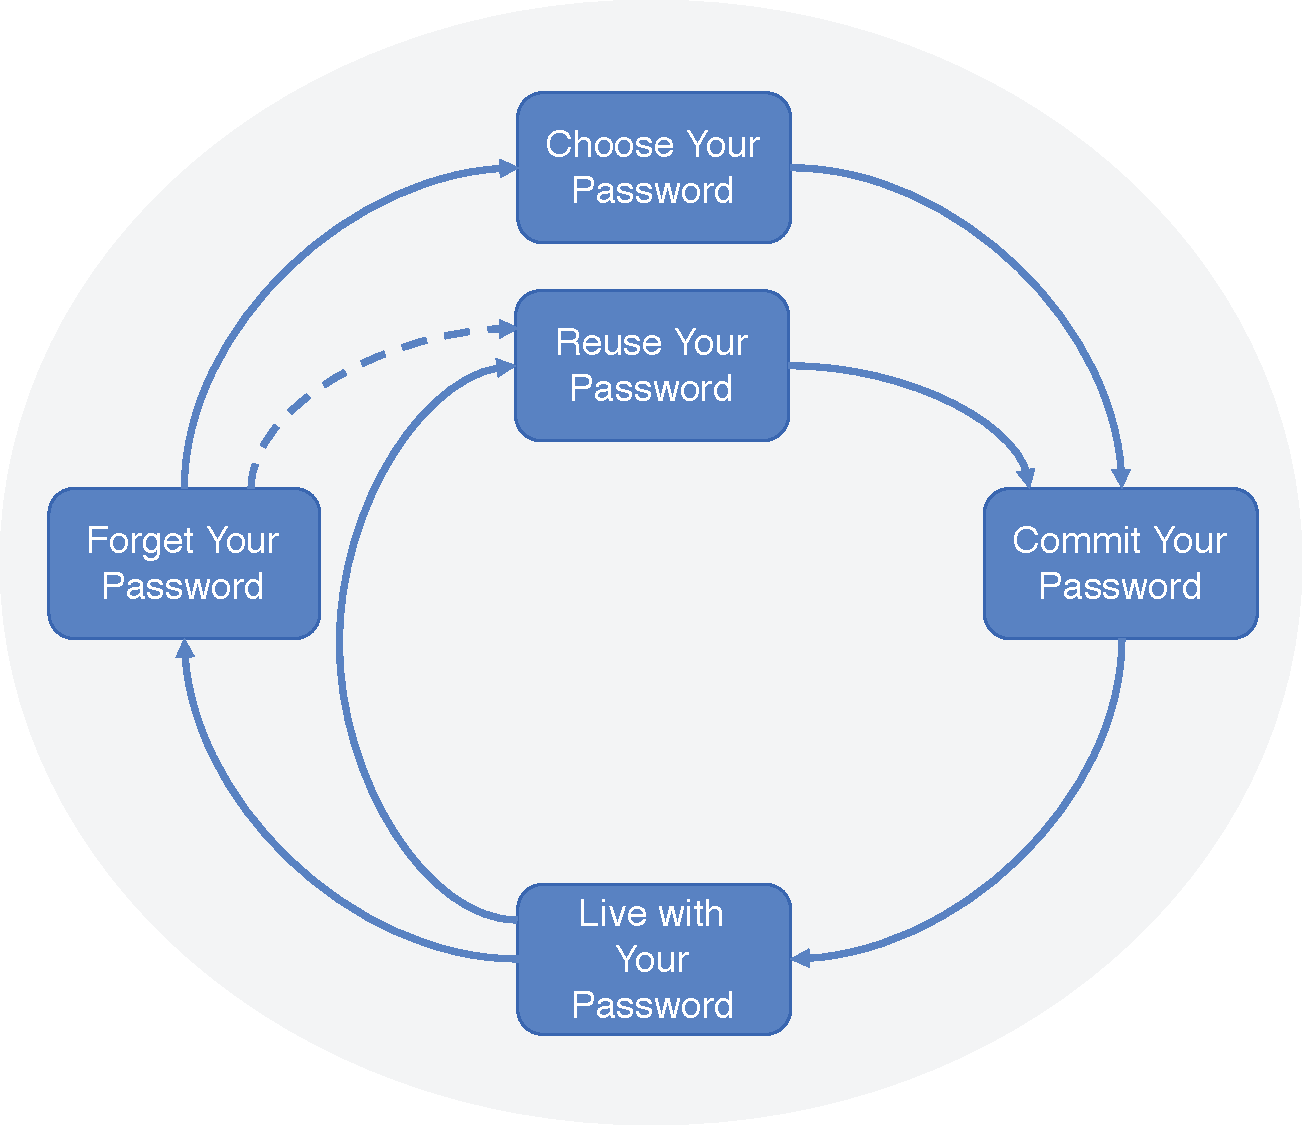
\includegraphics[width=0.65\linewidth]{rw/pw-life-cycle-new}
	\caption{\label{fig:rw:pw_life_cycle} Stobert and Biddle's ``Password Life Cycle'' \cite{Stobert2014PasswordLifeCycle} models typical stages of password behavior.}
\end{figure}

%TODO optional \todo{add a table that has all problems on one side and the possible user coping strategies on the other side.}

	\subsection{Selecting Weak Passwords}
	% things to answer in this section:
	% what's so difficult about selecting a strong password?
		% users do not see their passwords as predictable
		% users are too lazy. 
		% misconceptions about strength
	% what do users do if they want to select a strong password?
	% why don't they always do it?
	% when do they select stronger passwords?
	Why do users select weak passwords? 
	First of all, selecting a strong password is hard for most people. % I feel this lacks a reference ?
	Picking up the definition of a strong password (``something that is easy to remember, but difficult to guess'' \cite{Bishop1995ProactivePasswordChecking}), users do not struggle with the first part of the sentence, but the latter. Users do not intuitively know what makes a password \textit{difficult to guess} \cite{Jakobsson2013BenefitsUnderstandingPWs}, and not even security researchers reach ultimate consensus on that matter. 
	
	Let us look at the first part: something that is easy to remember. Numerous studies have looked at what people do to make their passwords easy to remember. For instance, personal information is easy to remember (``\texttt{TobiasSeitz}''), as is that of close ones (``\texttt{LenaSeitz}'') and pets (``\texttt{Fonsi\&Alois}'') \cite{Brown2004GeneratingPWs}. Looking at the top 10 most-used passwords\footnote{SplashData publishes such a list each year, for 2017: \url{http://fortune.com/2017/12/19/the-25-most-used-hackable-passwords-2017-star-wars-freedom/} \la{12.01.2018}}, a list published after each public data leak, we can easily spot more patterns.
	
	In theory, one could simply generate a random string of characters (see Section \ref{sec:rw:pwm_generators}), but those are not memorable. 
	Looking at the statistics of prominent password leaks (see Table \ref{tab:rw:password_leaks}), a large part of them are predictable. 
	
	pass\textit{word} implies it has to be a word. Other names for the concept, but basically the same meaning: security code, passcode, secret, credentials, access token
	
	\cite{Jakobsson2013BenefitsUnderstandingPWs}
	
	People show predictable modification behavior \cite{Gaw2005ReuseRecycle}
	
	a lot of RockYou's passwords are based on dates and this can be visualized and used for attacks \cite{Veras2012VisualizingSemanticsPasswords}
	
	Greek users do not behave differently than the rest, but the top 100 passwords are a bit different \cite{Violettas2014PasswordsAvoidGreece}
	
	
	\cite{Li2017PersonalInformation}
	
	
	\begin{figure}[htbp]
		\centering
		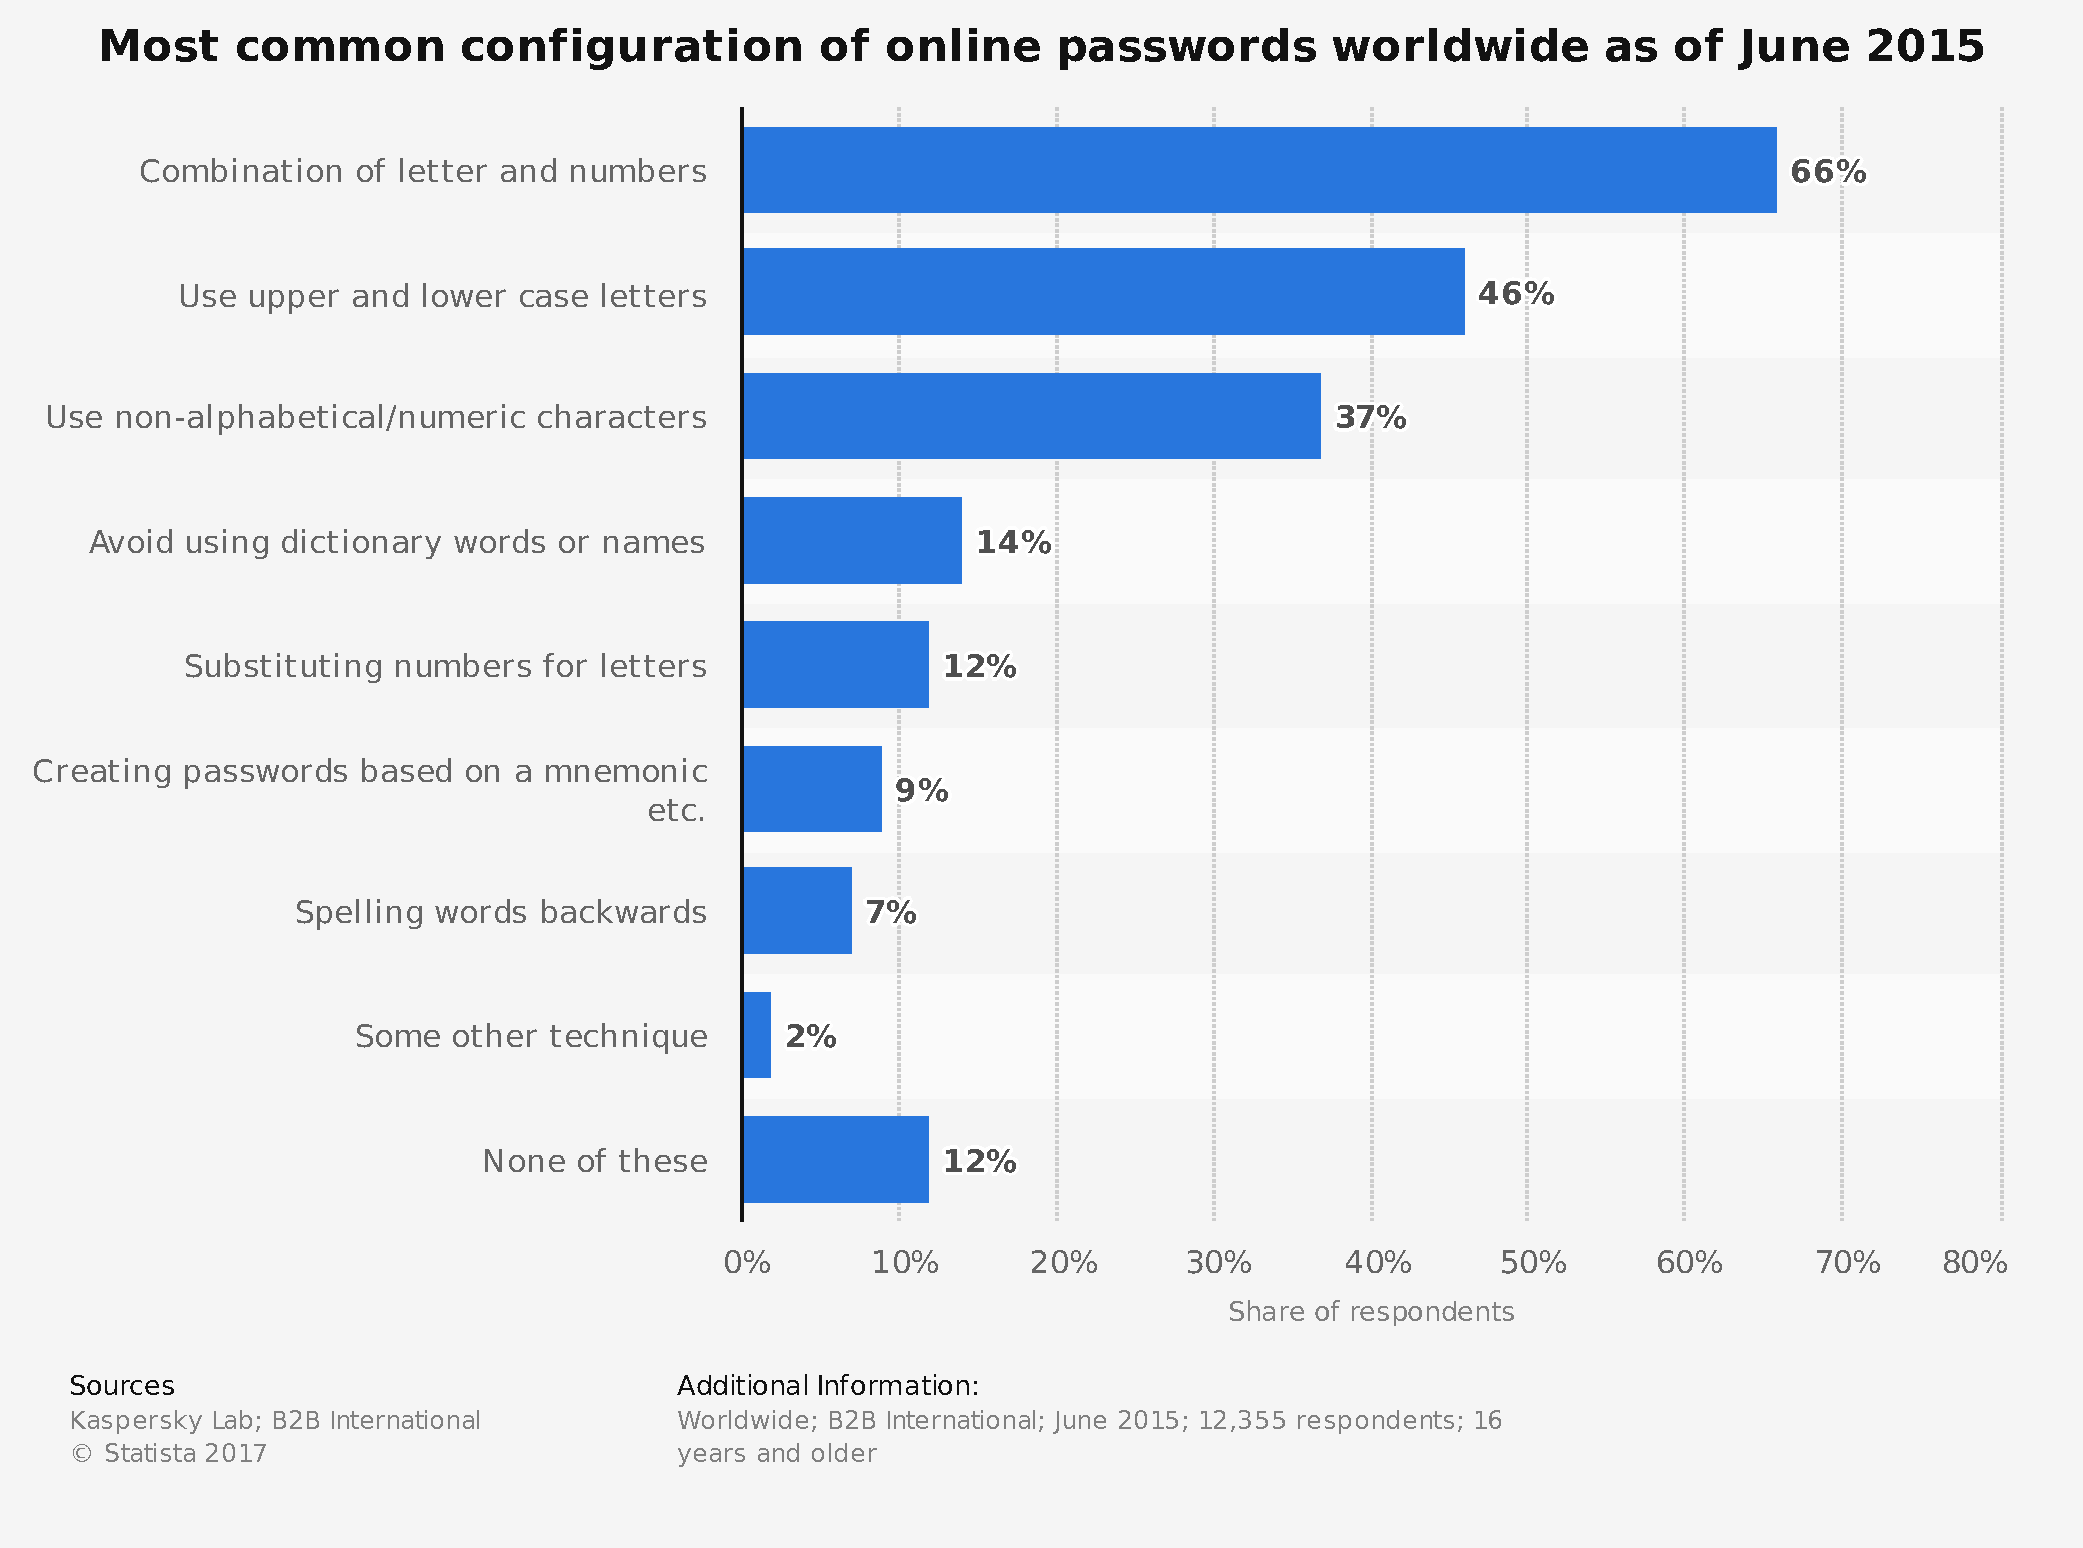
\includegraphics[width=0.6\linewidth]{../statista/statistic_id463406_typical-configuration-of-internet-passwords-2015}
		\caption{\todo{replace with own figure built from Kaspersky Lab report data} Survey results - how do people select their passwords (self report)}
	\end{figure}

	\subsubsection{Why do Users Select Weak Passwords?}
	
	Users act insecurely because they choose weak passwords that they reuse \cite{Riley2006WhatUsersKnowWhatTheyDo}
	
	people don't take password policies at organizations seriously.  \cite{Weirich2005PersuasivePasswordSecurity}
	
	- policies allow it (\cite{Seitz2017PoliciesReuse})
	- wrong mental model or misinterpretation of security advice (\cite{Ur2015PWCreationLab, Ur2016PerceptionsPassword, Seitz2017PASDJO})
	- because they don't care
	- They looked at depletion levels and password strength, but the method was kind of flawed so it's difficult to take this seriously \cite{Gross2016EffectCognitiveEffort}
	- ... they underestimate the threat
	- ... they are right to judge the account as low value (who would hack me?) \cite{LastPass2016PersonalitiesGetUsHacked}
	- Passwords survive for a long time, sometimes in a modified version, and they tend to get slightly more complex over time and for important accounts\cite{VonZezschwitz2013SurvivalShortest}
	- people think complex passwords are not memorable enough \cite{Woods2018TooManyPasswords}
	
	Passphrases are super predictable because most people use common phrases \cite{Bonneau2012LinguisticProperties}
	
	\cite{Wang2015ChinesePWs}
	
	thesis on the ``why'': \cite{Notoatmodjo2007ExploringWeakestLink}
	
	qualitative studies \cite{Ur2015PWCreationLab, Stobert2014PasswordLifeCycle} 
	quantitative studies \cite{Ur2016PerceptionsPassword, Seitz2017PASDJO}
	
	
	Text entry under lab conditions for multiple password selection tasks in a row doesn't have a large effect on typical password metrics \cite{Yang2014EntryAffectsPasswordSecurity}
	
	input modality can be a strong influence on password selection in that mobile devices will lead to less diverse passwords \cite{VonZezschwitz2014HoneyIShrunkTheKeys}
	
	Users understand quite a bit about password security, but we should help them how attacks work \cite{Ur2016PerceptionsPassword}
	
	
	Users are not too bad at creating strong passwords, but often they misinterpret security advice which leads to weak password practices \cite{Ur2015PWCreationLab}
	
	Even after a credential leak people are not very invested with their weak passwords: LinkedIn's password reset email can be considered ineffective, but the more severe problem is that the email focused on LinkedIn only, because it's super important to change the password on all other sites \cite{Huh2017TooBusy}
	
	\subsubsection{What's the Problem with Weak Passwords?}
	usually, people tend to use stronger PWs for important accounts
	
	Stronger passwords are not always necessary, do not force users to waste effort. \cite{Florencio2007DoStrongWebPasswords}	
	
	\cite{Shay2014ReligiousAunt}
	
	\subsubsection{The Influence of Mobile Devices}
	touch some small aspects, especially Melicher's Paper \cite{Melicher2016UsabilityMobileTextPasswords} and \cite{VonZezschwitz2014HoneyIShrunkTheKeys}
	\cite{Haque2014PsychometricsStrongPassword} 
	
	talk about the rise of graphical and biometric authentication. 
	also \cite{Cherapau2015ImpactOfTouchID} -- fallback stuff.
	
	new character set: emojis.
	set the stage for the emoji passwords later. 

	\subsection{Password Reuse}
	too many accounts problem. ``password overload'' and ``memory interference'' as technical terms must appear here (for discussion see \cite{Yang2016MnemonicSentenceBased}). in the same vein: \cite{Chiasson2009InterferencesGraphical}
	
	People reuse their passwords and show predictable modification behavior \cite{Gaw2005ReuseRecycle}
	
	The burden of passwords was relatively high in 2007, people reuse passwords \cite{Florencio2007LargeScaleStudyPasswordHabits}: They found that users had about 7 distinct passwords in 2007, and that passwords are re-used at about 6 sites in average. Interestingly, they found that stronger passwords are not re-used as often as weak passwords (only around 4 sites). 
	
	finite effort, and the payoff is invisible (comparison to smoking: I won't be affected, and in many cases that's true. But if you are affected you regret your behavior. )
	
	reuse is the most convenient way but probably the most severe threat to one's online identity and finances. This is a hard problem. 
	
	it's not just the passwords, it's also the user name 
	
	frequently entered passwords are reused more often \cite{Wash2016UnderstandingPasswordChoices} -- but there are contradictory results on this matter. -- Stobert and Biddle argue in the other direction \cite{Stobert2014PasswordLifeCycle}. 
	
	reuse statistic overview of different papers: 
	\cite{Wash2016UnderstandingPasswordChoices} in the discussion section
	Users try to prioritize stronger passwords as reuse candidates, and this also means that users try to follow security advice (they belief strong passwords are more important than unique passwords) \cite{Wash2016UnderstandingPasswordChoices}
	
	term that you read ever so often: users have a ``go-to password'' that they try first
	and then often the policy can make them change another one. But! If the go-to password is strong and has certain characteristics (as is demonstrated in chapter \ref{chap:policies-reuse}), reusing this is possible and its threats perhaps underestimated. 
	
	\textbf{What's the problem?}
	consequences: phishing attacks are problematic because of the domino effect (Ives \etal) Password reuse is difficult to defend against and we should look into understanding user behavior better \cite{Ives2004DominoEffectReuse}.
	
	but reuse isn't bad per se, it's necessary \cite{Florencio2014PasswordPortfoliosFiniteUser, ZhangKennedy2016RevisitingPasswordRules}. 
	

	
	
	It's enough to know one low-value password that you mangle to crack a large part of high-value passwords \cite{Haque2014Hierarchy}
	
	
	%    \subsubsection{Reuse Strategies}
	address the role of policies (see \cite{Seitz2017PoliciesReuse}).
	
	Participants rely on their memory, but reuse passwords, and they have a suboptimal mental model of how attacks work \cite{Gaw2006PasswordManagement}
	
	Users don't care if an account is financial or not, as long as it's perceived as high value, they reuse the password for that \cite{Bailey2014StatisticsReuse}
	
	password reuse is common and modifications are predictable, so it's easy for attackers to optimize their attacks with knowledge from leaked credentials of a specific account \cite{Das2014TangledWeb}

	Password Categories -- arch over to mental accounting from behavioral economics -- \cite{Thaler2004}
	
	Experts have certain articulate strategies to select and manage their passwords, and their situation awareness lets them judge important and non-important accounts more consistently  	\cite{Stobert2015ExpertPassword} 
	but: not all of them behave the same way \cite{Loutfi2015PasswordsOtherSideOfTheFence}

	Categorization: 
	compare password categorization to mental accounting, then we can cite \cite{Stockinger2015TowardsBE}
	
	category: depending on policies. \cite{Stobert2014PasswordLifeCycle}
	
	
	``Users see `good' passwords (that are memorable and conform to the policy) as a `resource', which they continue to use for new applications even if the original use is no longer allowed.'' (\cite{Inglesant2010TrueCostOfUnusablePolicies})
	
	Users try to prioritize stronger passwords as reuse candidates, and this also means that users try to follow security advice (they belief strong passwords are more important than unique passwords) \cite{Wash2016UnderstandingPasswordChoices}.
	
	Coping with passwords by choosing weak passwords and reusing them is absolutely necessary, the problem is how to do it right \cite{Florencio2014PasswordPortfoliosFiniteUser}.
	
	A new scale and insights into password support. Password hierarchy \cite{Haque2015PhdProposal}
	
	\subsection{External Storage}
	
	%Write down passwords.
	\cite{Herley2012PersistenceOfPasswords} is in favor of writing down IF the location is secure enough.
	
	Users struggle to manage passwords, but are unfamiliar with supporting tools, so they have developed elaborate strategies to cope \cite{Stobert2014Agony}
	
	Many people like using a password logbook and have interesting motivations to do so \cite{Kothari2017PasswordLogbooks}
	
	\cite{Conklin2004PWAuthenticationSystemPerspective}
	
	Problem: Accessibility for Local Attackers
Word documents post-its (use a screen shot of french newspaper that was featured on tv and you could see one of their passwords in the back. spouses can access them .	


	\subsection{Fallback Methods}
	Click on ``forgot'' password basically every time - to avoid this, some services mainly rely on one time passwords, because users are going to forget theirs anyway. 

	\cite{Bonneau2015SecretsLies}
	


	\subsection{Account Sharing}
	Account sharing is very common and often necessary, while current designs do not take this behavior into account \cite{Singh2007PasswordSharing}

	\subsection{Summary}
	This is where the password life cycle plays an essential role \cite{Stobert2014PasswordLifeCycle}
	
	FINITE USER EFFORT advocates the rationality of these coping strategies. 

%%%%%%%%%%%%%%%%%%%%%%%%%
%%%%%
%%%%% COUNTERMEASURES
%%%%%
%%%%%%%%%%%%%%%%%%%%%%%%%
\section{Countermeasures}

if we must keep the human in the loop, e.g. because constraints dictate so, we need to support them well and carefully \cite{Cranor2008FrameworkReasoning}

Usable security shouldn't only be done for end users but also for the people who implement security systems \cite{Acar2016NotYourDeveloper}


	\subsection{Password Composition Policies}\label{sec:rw:policies}
	
	
	
	
	the idea of policies dates back to the 70s: Morris and Thompson suggested to make users
	either choose longer passwords or assign passwords to them - There are flaws in password authentication and we can do something to alleviate the problem, but cannot get rid of it entirely \cite{Morris1979PasswordSecurity}
	
	The algorithms at the time weren't suitable to defend against cracking attacks so it was thought to introduce a few mechanisms to shift responsibility to the users \cite{Feldmeier1990UnixPasswordSecurity}
	
	%TODO here we need a reference to Bill Burr's idea of nailing policies down to a NIST standard.



	Proctor \etal found in 2002 that certain ``proactive password restrictions'' lead to stronger passwords \cite{Proctor2002ImprovingAuthenticationProactivePasswordRestrictions}. In two laboratory experiments, they had participants create a new password for a university account. The policies differed in the required minimum length (five and eight) and additional requirements like upper-/lowercase letters and digits. In the first experiment, where passwords only had to be five characters long, introducing the additional requirements had a greater effect on strength than in the eight-character-minimum condition. Increasing the minimum length by three characters already had a stronger effect. Interestingly, they concluded ``Perhaps the most important message of this study is that restrictions on user-generated passwords may not accomplish their intended goals.'' 
	
	%TODO NIST policy derived from their guessing approach in 2004. 
	%% also mention that Bill Burr regrets putting it out there!
	
	Proctor \etal's early hypothesis that policies are more or less ineffective is particularly surprising because in the fifteen years that followed, many research papers were written about such restrictions and many of them ultimately came to similar conclusions. In the following some of the most influential works are summarized.
	
	%now we need to report on a couple of papers that come to the conclusion that policies are somewhat ineffective.	
	Inglesant and Sasse report on a diary study of password policies in corporate contexts \cite{Inglesant2010TrueCostOfUnusablePolicies}. a postulation that password policies should be based on HCI principles rather than security considerations alone. The idea of a holistic password policy is put forward 
	
	 
	
	%Lingo: Adhere to a policy
	

	
	
	Weir \etal categorize policies into ``explicit'' and ``implicit'' policies \cite{Weir2010MetricsPolicies}, where explicit policies have predefined rules about the password structure (e.g. LUDS policy). Implicit policies are based on the estimated strength and are somewhat more volatile and intransparent to the users. Example: blacklist only becomes visible once the user tries to pick a password that's contained in the list. There are also ``external'' policies where the user's password is automatically changed by the system to add some randomness
	
	
	Policies influence security and usability, meters are often ineffective because only stringent meters seem to work \cite{Ur2012HelpingUsersCreateBetterPasswords}
	
	LUDS as a key term \cite{Wheeler2016zxcvbn}
	
		
	Range of Policies as shown by Shay \cite{Shay2014CanLongPasswordsBeSecureAndUsable}
	definitely mention: 28.0\% of passwords in comp8 fulfilled the symbol requirement only by placing ``!'' at the end and using no other symbols. 
	
	Zhang-Kennedy 2016 (here and also below) \cite{ZhangKennedy2016RevisitingPasswordRules}
	
	
	Workplace-focused: 
	
	
	The authors present how they would design an experiment about persuasive messaging, but didn't really carry it out (and the method doesn't seem suitable) \cite{Zakaria2013DesigningEffectiveSecurityMessages}
	
	Don't try to fix the user, fix the system first, especially do not impose strict requirements and nonsensical policies \cite{Florencio2014AdministratorsGuide} 
	
	Policy changes are a nuisance, but users feel more secure afterwards, and users write down passwords, share them and base them on dictionary words 	\cite{Shay2010EncounteringPasswordRequirements}
	
	Most detailed insights into effects of password policy design we have to date, password substring blacklist suggestion \cite{Shay2016DesigningPasswordPolicies}
	
	\cite{Weir2010MetricsPolicies}
	
	\cite{Wang2015EmperorsPolicies}
	
	
	\cite{Florencio2010WhereDoPoliciesComeFrom}
	
	\cite{Horsch2016PasswordPolicyMarkup}
	
	\cite{Chiasson2015QuantifyingExpiration}
	\cite{Blocki2013OptimizingPasswordPolicies}
	
	Early comparison of the effects of policies on \textit{human} password selection by Komanduri \etal - A carefully chosen policy can lead to more secure and more usable passwords, in this case the basic16 policy was well-received \cite{Komanduri2011OfPasswordsAndPeople}
	
	
	Shay tried to come up with an algorithm that lets administrators decide which policy to use - We could pick a password policy algorithmically based on a number of variables in this context \cite{Shay2009PolicySimulation}.
	
	basic16, 3class12, and 2word16 seem like the winners in terms of security and usability, but persuasion can help to diversify the themes for word-based passwords \cite{Shay2014CanLongPasswordsBeSecureAndUsable}
	
	
	Penalizing users by making them wait can be a strong nudge to comply and create a stronger password \cite{Malkin2013Waiting}
	
	It would be nice to have an easy way to create a repository with all password policies, but it isn't easy - at least it helps to agree on a standard language to define a password policy \cite{Steves2015PasswordPolicyLanguage}
	
	It would be good to have a formal description of password policies in a standardized schema \cite{Horsch2016PasswordPolicyMarkup}

	\subsection{Training, Advice, and Guidelines}\label{sec:rw:advice_guidance}
	
	there is a plethora of advice and guidelines out there, but it's not all the same \footurl{https://www.ncsc.gov.uk/guidance/helping-end-users-manage-their-passwords}{22.12.2017}
	
	education in password matters only has so much effect. 
	\cite{Forget2007HelpingUsers} says that even instructions don't work
	
	There's some work that argues that users want to create stronger passwords at least for some accounts, but they had
	misinterpreted security advice. 
	this is also reflected in \cite{Ur2016PerceptionsPassword}
	
	Great overview and critical discussion: \cite{ZhangKennedy2016RevisitingPasswordRules}
	
	Example for training \cite{Bonneau2014ReliableStorage56Bits}
	
	make it persuasive \cite{Zakaria2013DesigningEffectiveSecurityMessages}
	
	In privacy: people's mental models about privacy are vague and we can see it in their drawings/explanations that they're somewhat overly pessimistic and that education plays the major role \cite{Kang2015MentalModelsDrawing}
	
	
	Stay realistic about password requirements and user effort \cite{Florencio2016CommACM}
	
	We can give better recommendations to users that are appropriately secure, actionable and usable \cite{ZhangKennedy2016RevisitingPasswordRules} (maybe also mention in policy section)
		
	
	\subsection{Offering Memorization Techniques}
	
	%TODO some papers actually could be categorized as password generator papers (semi-involved with human password selection.)
	
	early approaches: random but pronounceable passwords. (good overview in \cite{Kuo2006HumanSelectionMnemonic})
	
	\cite{Bonneau2014ReliableStorage56Bits}
	\cite{Forget2007HelpingUsers}
	Sort of displaced here, but it might be discussed in Section \ref{sec:rw:authentication_without_pws} \cite{Forget2015CYOA}
	\cite{Brown2004GeneratingPWs}
	
	In a convenience sample, persuasive text passwords were sufficiently memorable \cite{Forget2008MemorabilityPersuasivePasswords}
	
	It might be worthwhile to add a gamification layer onto password managers if you want to memorize some of your most important passwords \cite{Kroeze2012GamifyingAuthentication}
	
	They proposed a model to securely generate site-specific passwords, but this is all just an idea \cite{Maqbali2016PasswordGenerators}
	
	
	Security-wise this maybe a good idea, but the actual implementations is not as usable as it could be, however letting users modify system-assigned passwords seems beneficial in general \cite{Huha2015UserReplaceablePasswords}
	
	\paragraph{Mnemonics}
	Using contextual cues related to a website to base a mnemonic PW on might make them more memorable \cite{Mcevoy2016ContextualizingMnemonicPhrase}
	
	Yet another memorization aid - work in progress \cite{Lyastani2016PWMangling} 
	
	Even mnemonic phrase based passwords can be attacked easily, but if you tell people to choose something personal that no one else would choose and give an example might be the best piece of advice \cite{Yang2016MnemonicSentenceBased}
	
	People's mnemonic passwords are predictably based on common phrases from movies, literature, etc., but still the resulting passwords are better than traditional passwords \cite{Kuo2006HumanSelectionMnemonic}
	
	\paragraph{Passphrases}\label{sec:rw:passphrases}
	(\todo{maybe even merge this with subsection on advice})
	Advantages: PW scheme doesn't have to be changed, people are generally familiar with the concept of passwords, better to enter on virtual keyboards, e.g. TVs (although we don't have any data for that, but that's okay because passwords play a minor role (but still exist there)).
	
	Mnemonic phrase based passwords are strong and memorable \cite{Yan2004PasswordMemorabilitySecurity}.
	
	\cite{Keith2009PassphraseDesign}
	
	Disadvantages: more typos (can be relieved by displaying the password in plain text  \cite{Melicher2016UsabilityMobileTextPasswords}), user choice often predictable
	
	users might not even understand what you want from them if you say they should create a password based on a phrase \cite{Forget2007HelpingUsers}
	
	\cite{Bonneau2012LinguisticProperties}: passphrases already deployed in PGP, Caine and Abel password leak \cite{Carnavalet2014AnalyzingPWStrengthMeters} 
	
	\cite{Shay2012CorrectHorseBatteryStaple}
	
	
	\paragraph{Pronounceable Passwords}
	pronounceable passwords are useful, but we don't know the best way to generate them \cite{Goldberg2015UnspeakablePasswords}
	
	
	\subsection{Password Meters and Real-Time Feedback}
	
	\todo{Define what we mean by password meter} Because some papers don't differentiate between the meters, verbal feedback, suggestions, and real-time feedback on policy fulfillment. (this will be good to show with examples from the real world.)
	
%	Shay \etal say that real-time feedback is not part of the password meter \cite{Shay2015SpoonfulOfSugar}
	
	
	History: zxcvbn paper has some intel on early work on proactive password checks (in the 80s) \cite{Wheeler2016zxcvbn}. specifically (from 1995) \cite{Bishop1995ProactivePasswordChecking}
	
	
	pro-active checks -- dictionary checks Shay argues in favor of dictionary checks \cite{Shay2014CanLongPasswordsBeSecureAndUsable} 
	black lists \cite{Habib2017Blacklists} 
	
	spoonful (guidance) \cite{Shay2015SpoonfulOfSugar}
	\cite{Forget2008ImprovingPasswordsThroughPersuasion}
	
	be careful not to talk too much about persuasion in this chapter. 
	
	We should consider social nudges in usable security, too \cite{DiGioia2005SocialNavigationUsableSecurity}
	
	
	A sudden surge of n-gram scores can be used to detect modifications of common/weak passwords \cite{Tupsamudre2016MarkovStrength}
	
	
	passwords created using telepathwords were stronger and still memorable, but some Ps didn't like the idea \cite{Komanduri2014Telepathwords}
	
	Password meters from the industry are bad, machine-learning meters are good \cite{Wang2016fuzzyPWM}
	
	Users can well estimate the strength of their passwords, and can be nudged to act more securely for important accounts, but not for unimportant stuff \cite{Egelman2013DoesMyPasswordGoUpToEleven}
	
	Meters have a small effect on password strength, but slightly annoy people and it doesn't really matter how they look \cite{Ur2012HowDoesYourPasswordMeasureUp}
	
	Preliminary work to Ur et al.'s data-driven password meter \cite{Eargle2015YouCanDoBetter}
	Use text feedback to craft more effective password meters, but this depends on the policy used \cite{Ur2017DataDrivenPWMeter}
	
	If you tell people how long it will take to crack their password, they are more likely to read your recommendations and modify their password \cite{Vance2013FearAppeals}
	
	Password meters score the same password very inconsistently and don't explain their scoring, and it seems the Dropbox meter is one of the better solutions \cite{Carnavalet2014AnalyzingPWStrengthMeters}
	
	the presentation of password requirements can affect usability and security, because it can prevent errors and speed up selection for some stricter policies \cite{Shay2015SpoonfulOfSugar}
	
	time to crack already in \cite{Yee2006Passpet} for master password in PWM
	
	%TODO Move persuasion topic in here! maybe sort password meters (and managers sort of) in there. 
	
	\subsection{Password Managers and Generators}\label{sec:rw:pwm_generators}
	
	You give up control, if you generate random passwords. 
	Password managers that do ``autofill'' have the nice side effect of reducing susceptibility to phishing attacks (domain mismatches, so it won't autofill on phishing sites. only if the site was attacked with XSS (form action redirect) the pwm is fooled to autofill. )
	
	Goals of password managers see \cite{Yee2006Passpet}
	
	Generators and generative approaches
	\begin{figure}
		\centering
		%TODO we could use Dashlane's screenshot here. 
		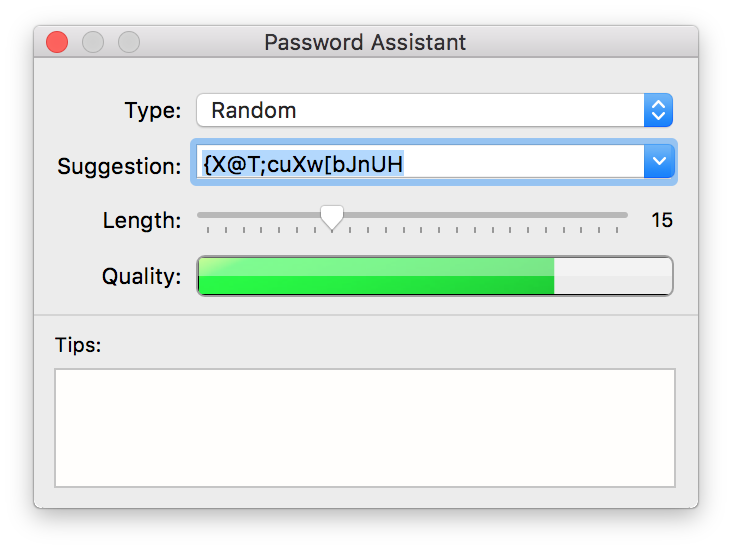
\includegraphics[width=0.49\linewidth]{rw/apple-pw-assistant-random}
		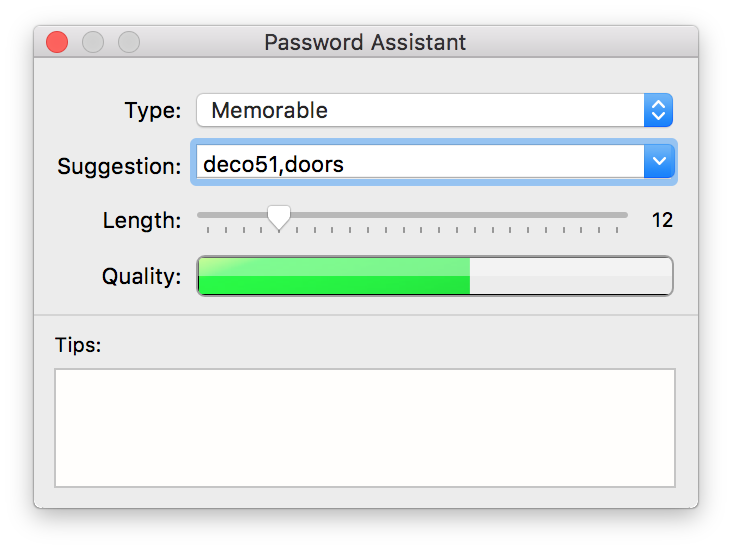
\includegraphics[width=0.49\linewidth]{rw/apple-pw-assistant-memorable}
		\caption{\label{fig:rw:pw_generators} On macOS, the Keychain application manages passwords for the user. If a new entry is manually created by the user, the password assistant can be used to generate different kinds of passwords: Random (image on the left), letters and numbers, numbers only, memorable (image on the right), and FIPS-181 compliant}
	\end{figure}
	
	Lyastani \etal recently investigated the impact of using a PWM on password strength and reuse \cite{Lyastani2017ImpactPWMPasswordStrength}
	
	list all the pro's and con's of PWMs here in different dimensions, e.g. security and usability, kind of similar to \cite{Bonneau2012ReplacePasswords}
	
	Dashlane has the best usability and security tradeoff - but the usability evaluation is kind of worthless without more background information \cite{AriasCabarcos2016ComparingPWM}
	
	Tapas is a password manager based on two-factor authentication and was well received in a 30/10 participant user study \cite{McCarney2012Tapas, McCarney2013PWMThesis}
	
	Passpet \cite{Yee2006Passpet}
	
	VersiPass \cite{Stobert2014PWMThatDoesntRemember}
	
	Password Multiplier \cite{Halderman2005ConvenientPWM}
	
	Drawbacks: Single point of failure, security problems\footurl{https://www.businesswire.com/news/home/20151006006149/en/Latest-Data-Breach-Spotlights-Identity-Restoration}{11.01.2018} 
	
	%% from SOUPS MM Poster
	We situate our work in understanding user behavior and attitudes regarding passwords. Here, large parts of the literature focus on \textit{coping strategies} that emerge with a growing number of accounts \cite{Florencio2007LargeScaleStudyPasswordHabits, Florencio2014PasswordPortfoliosFiniteUser}. For example, Stobert and Biddle conducted qualitative analyses to formalize the way users live with their passwords (the ``Password Life Cycle'') \cite{Stobert2014PasswordLifeCycle}. This model depicts how users choose, commit, reuse, and reset their passwords. Their work also delivers valuable insights into memorization and organization strategies: Users have mental lists of passwords, e.g. a list for important accounts or a list per website topic. Without explicitly mentioning, the findings contribute to a mental model of password reuse. This is important, because reuse is one of the most common coping strategies \cite{Das2014TangledWeb, Gaw2006PasswordManagement, Hayashi2011DiaryStudyPWs} and many researchers discourage it, because a breach at one site can compromise many others \cite{Bonneau2012ScienceOfGuessing, Komanduri2011OfPasswordsAndPeople}. 
	
	To facilitate coping with passwords and possibly minimize reuse, dedicated tools have been investigated and proposed. Besides industry-driven password managers, HCI research has proposed a number of alternatives. For instance, Stobert and Biddle also propose a password manager that is designed to boost trust as it does not directly store passwords, but rather offers a image cues to recall passwords \cite{Stobert2014PWMThatDoesntRemember}. 
	
	
	\cite{Bojinov2010KamouflagePWM}
	
	\cite{Fagan2017UsersConsiderationsPWMs}